%-------------------------------------------------------------------------------
% yum_configuration
%-------------------------------------------------------------------------------
%
% \file        yum_configuration.tex
% \library     Documents
% \author      Chris Ahlstrom
% \date        2016-03-07
% \update      2018-05-26
% \version     $Revision$
% \license     $XPC_GPL_LICENSE$
%
%     Provides descriptions of the configuration files.
%     Not yet part of the document.
%
%-------------------------------------------------------------------------------

\section{Configuration Files}
\label{sec:configuration}

   Let's cover the configuration files, which have expanded in utility in
   recent versions of \textsl{Yoshimi}.
   Understanding these configuration file makes it easier to
   use \textsl{Yoshimi}.
   Also note that all configuration settings are exposed to the command line
   interface as well.

   As with most applications, \textsl{Yoshimi} and \textsl{ZynAddSubFX}
   allow for one to save one's work and reload it.
   In recent versions of \textsl{Yoshimi}, it is possible to autoload a default
   state on startup, so that \textsl{Yoshimi} is already configured exactly as
   desired, with patches loaded and part destinations set.
   In addition, \textsl{Yoshimi} now saves settings that have been disabled.
   In this way, they can be re-enabled without having to reconstruct them from
   scratch.

   However, the configuration has changed quite a bit, and configurations from
   \textsl{Yoshimi} 1.4 and earlier will need to be reconstructed.  The
   following warning will occur if that is the case:

\begin{figure}[H]
   \centering
   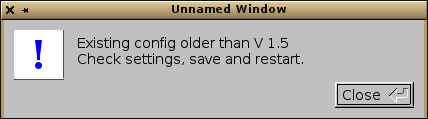
\includegraphics[scale=0.75]{1.5.0/ConfigWarn.png}
   \caption{Configuration Warning Dialog}
   \label{fig:config_warn_dialog}
\end{figure}

   \textsl{Yoshimi} has a number of different files that make up the current
   configuration.
   Together, they make up the concept of a \textsl{patch set} (also called a
   \textsl{patchset}).
   Sometimes one will see reference to a "session", but that term is too easy
   to confuse with the "session" in "JACK session manager".
%  Here are the file extensions used for saving the \textsl{Yoshimi}
%  patch-set data:

   The last-used file in any configuration section is always at the top of its
   history list.  The main benefit of this new setup is that now all patch
   sets, vectors, scales, MIDI Learn, and state - offer the most recent entry
   when asked to load or save. On first-time use, when there is no history, one
   is offered one's home directory as a location, regardless of where
   \textsl{Yoshimi} was called from.  Presets are not yet included in this
   process.

   When saving these "managed" files, one won't be offered the previous
   last-used configuration unless it was seen during that session, either by
   being loaded, or saved by name.  This protects against accidental
   overwrites: you've been working on 'foo' for a whole day, saving as you go,
   then the following day you start up \textsl{Yoshimi}, and immediately have
   a completely new idea 'bar', and start working on it. Without thinking you
   save and hit Enter. Oops, you just wiped out 'foo'. Only now you haven't,
   because while loading \textsl{Yoshimi} would see the older file, so the
   save command just offers the home directory to put a new name in.

   Here is a summary of the files.  Please note that the names all start with
   \texttt{yoshimi}.  For example, \texttt{.banks} is really
   \texttt{yoshimi.banks}.

   \begin{itemize}
      \item \texttt{.banks}
         \index{.banks}
         \index{config!.banks}
         Contains information on the accessible instrument banks, and
         information to translate between bank directory names and bank ID
         values.
         Current root and current bank settings have now been moved from
         \texttt{banks} to the \texttt{config} and \texttt{instance}
         files, so the banks file now consists only of the bank structure.
         On first time start up, \textsl{Yoshimi} will look for
         \textsl{ZynAddSubFX} banks as well as \textsl{Yoshimi} banks in the
         usual locations. It \textsl{will not} look for a \textsl{ZynAddSubFX}
         configuration file, as these are no longer relevant.
      \item \texttt{.config}
         \index{.config}
         \index{config!.config}
         Contains the setup information configured in the
         \textbf{Yoshimi / Settings} dialog.
         This is the main configuration file.
         Configuration instances are now in place, so the main configuration
         file is common to all, but each instance has its own file for things
         like current bank, JACK/ALSA settings, etc.
         Common settings are only visible
         in the main instance and completely hidden in all the later ones.
      \item \texttt{.history}
         \index{.history}
         \index{config!.history}
         Recent patch sets are now stored in the \texttt{.history} file.
         The last-used file in any section is always at the top of its history
         list.
      \item \texttt{\textasciitilde/.yoshimi\_history}
         \index{\textasciitilde/.yoshimi\_history}
         Holds command-line history, which is then available on the next
         \textsl{Yoshimi} session.
      \item \texttt{.instance(n)}
         \index{.instance(n)}
         \index{config!.instance(n)}
         Contains the current root/bank, MIDI settings, and preferred engines.
         \textsl{Yoshimi} now has instance data separated from the main
         configuration file, with the name \texttt{yoshimi-(n).instance}.
      \item \texttt{.state}
         \index{.state}
         \index{config!.state}
         Contains the state information needed to
         duplicate a \textsl{Yoshimi} session that was saved.
      \item \texttt{.windows}
         \index{.windows}
         \index{config!.windows}
         Contains the current layout of windows for reinstantiation at the next
         startup of \textsl{Yoshimi}.
         If there is no such file
         (\texttt{\textasciitilde/.config/yoshimi/yoshimi.window}) at
         \textsl{Yoshimi}, then the keyboard is also opened, alongside the main
         window, as a help to those new to \textsl{Yoshimi}.
         And of course that state will be saved, if present, when
         \textsl{Yoshimi} exits.
      \item \texttt{.xiz}
         \index{.xiz}
         \index{.xiz!Legacy format}
         \index{config!.xiz}
         An Instrument file.  This format is the \textbf{Legacy} or \textbf{Zyn}
         file format.  This format will be supported forever, although some
         backward-compatible refinements might be made as time goes on.
      \item \texttt{.xiy}
         \index{.xiy}
         \index{.xiy!Yoshimi format}
         \index{config!.xiy}
         An Instrument file in the new \textsl{Yoshimi} file format.
         This format includes all the
         controllers, the part mode status (Poly, Mono, Legato) and the
         Humanise setting.
         When loading files, \textsl{Yoshimi} will always look for
         the \texttt{.xiy} version first, and,
         if it can't find it, will then look for the \texttt{.xiz} version.
      \item \texttt{.xly}
         \index{.xly}
         \index{config!.xly}
         \index{MIDI Learn!.xly}
         A MIDI-Learn file for saving the MIDI-Learn settings in force at the
         moment this file is saved.  It is also included in the state file
         (\texttt{.state}).
      \item \texttt{.xmz}
         \index{.xmz}
         \index{config!.xmz}
         A full \textsl{Yoshimi} configuration; everything.
         This file is also called a \textsl{patch set}.
      \item \texttt{.xpz}
         \index{.xpz}
         \index{config!.xpz}
         Presets.
         A preset is a \textsl{Yoshimi} sub-setting file.
      \item \texttt{.xsz}
         \index{.xsz}
         \index{config!.xsz}
         Scale Settings.
      \item \texttt{.xvy}
         \index{.xvy}
         \index{config!.xvz}
         Vector settings. The extension stands for "Xml Vector Yoshimi".
         Vector settings are now included in both the patch sets
         (\texttt{.xmz}) and state files (\texttt{.state}.
         For a good example, see \sectionref{subsection:vector_command_line}.
         Vector control settings are now also stored in patch set and state
         files.
   \end{itemize}

   The entire config set should then be (ignoring the prepended
   \texttt{yoshimi}):

   \begin{itemize}
      \item \texttt{.config}
      \item \texttt{.instance[n]}
      \item \texttt{.windows}
      \item \texttt{.history}
      \item \texttt{.banks} (this is currently per instance)
   \end{itemize}

   The \texttt{.windows} file is specific to the GUI, so doesn't figure in this
   scheme at all, but it is created or saved when one exits
   \textsl{Yoshimi}.

   In the file-save dialogs, the file extension is determined by the type of
   file being saved, and it doesn't matter if one enters the extension
   explicity, or not. If it's missing, or it is the wrong one, it will be
   replaced. This is actually true of almost all file saves, and has been for
   quite some time now.

   For vectors (in common with external instruments and patch sets),
   the configuration is saved to the user's home directory.
%  it's up to the user as to where to save.
%  The file filter generally defaults to the
%  either the user home directory, or if \textsl{Yoshimi} was launched from
%  userland, it's the directory it launched from. Then it's the normal
%  file browser selection.
   Once saved, \textbf{Vectors / Options / Recent} is your friend.

   \textsl{Yoshimi} can set up critical configuration settings to be writable
   only by the main instance, but readable (and used) by any others. In the
   current version of \textsl{Yoshimi}, this applies to \textbf{AddSynth
   Oscillator Size}, \textbf{Internal Buffer Size}, and \textbf{Alsa
   Samplerate}. These three must be defined before any other initialisation.

\subsection{Configuration Files / Patch Set}
\label{subsec:configuration_patch_set}

   \index{.xmz}
   \index{config!.xmz}
   \index{patch set}
   \index{file!patch set}
   A patch set is basically a group of instruments related simply by the user
   wanting to have them all loaded at once into \textsl{Yoshimi}.  A patch set
   is stored in a \texttt{.xmz} file.  A patch set is akin to a preset, in that
   it stores a combination of items, that took awhile to set up, for easy
   retrieval later.

   Patch sets are not the full configuration. They carry \textsl{most} of it,
   including almost all of the dynamic settings, but they don't contain the
   configuration settings that \texttt{.state} does.  The patch set format is
   either XML or compressed XML, as explained elsewhere.  The
   \textbf{Patch Sets / Save External...} menu entry saves files with
   the \texttt{.xmz} extension.

   One of the simplest ways to save one's work is to save the entire
   dynamic settings \textsl{Yoshimi} configuration.
   This saving can be done through the \textbf{Patch Sets} menu
   (the \textbf{File} menu in \textsl{ZynAddSubFX}),
   and will result in the creation of
   a \texttt{.xmz} file. Once created, this file will hold the settings for
   all settings within that setup, such as microtonal tunings, all
   patches, system effects, insertion effects, etc.
   See \sectionref{paragraph:menu_yoshimi_settings_main_settings}.
   Patch sets will save all other instruments regardless of whether they are
   activated or not.

   In many cases saving everything in a part is not what is desired.
   Saving a patch later on in an editing session is one such example.
   In order to save a patch, one can either save it from the
   \textbf{Instruments} menu, or through the \textbf{Bank} window.

\subsection{Configuration Files / Config}
\label{subsec:configuration_config}

   \index{.config}
   \index{config}
   \index{file!config}
   Often, one will see the extension \texttt{.config} used in the
   \texttt{\$HOME/.config/yoshimi} directory.  This file once contained
   information to translate between bank directory names and bank ID
   values.  In recent versions of \textsl{Yoshimi}, this file is much
   reduced in size, and its "doctype" is no longer "ZynAddSubFX".

   The \texttt{.config} file is always going to be specific to one machine and
   working modes, so no one will ever want to copy it across even to another
   \textsl{Yoshimi} environment.  Recent patch sets are now no longer stored in
   the main \texttt{.config} file, but in a new \texttt{.history} file.  The
   \texttt{.config} file is now a much reduced common settings -- interfaces,
   sample rate -- file.  It is a single file that every instance can read, but
   only the first one can write.

   The \texttt{.config} file has been separated from \texttt{.instance(n)}.
   It is saved only when the user explicitly calls for it to be saved.

   All files are still per instance, as the
   \textsl{Yoshimi} team haven't had time to work out exactly how to manage
   common files and memory locations for those that should be shared.
   \textsl{Yoshimi} will still mention its absense:

   \begin{verbatim}
      $ yoshimi -a -A
      Yoshimi is starting
      ConfigFile /home/ahlstrom/.config/yoshimi/yoshimi.config not found, will
         use default settings ...
   \end{verbatim}

   The \texttt{.config} file will be readable by all instances of
   \textsl{Yoshimi}, but writeable only by the main instance. The relevant
   controls will be hidden from the other instances.  Also, those controls not
   relevant to LV2 are disabled in that mode.  The \texttt{.config} and
   \texttt{.banks} data now reside in separate configuration files.  The banks
   file is saved every time there is a normal exit, so the last-used root and
   bank IDs will always match what that instance thinks is there.  Conversely,
   the main \texttt{.config} file \textsl{doesn't} get saved when one starts a
   new (unkown) instance of \textsl{Yoshimi}, but the config-changed flag is
   set, so one has control over whether any settings are saved.  So now, if
   anything goes wrong with the config files they won't corrupt one's carefully
   organised bank files, and vice-versa.

\subsection{Configuration Files / State}
\label{subsec:configuration_state}

   \index{.state}
   \index{config!.state}
   \index{state}
   \index{file!state}
   Sometimes one will see the extension \texttt{.state} used in the
   \texttt{\$HOME/.config/yoshimi} directory.  These files contain a lot more
   information, that needed to duplicate a \textsl{Yoshimi} session that was
   saved.  This file is a superset of an \texttt{.xmz} file, saving everything.
   The state file is accessed from the \textbf{State} menu item in the main
   window.
   Its default name is
   \texttt{\textasciitilde/.config/yoshimi/yoshimi.state}.
   This file is auto-loaded when \textsl{Yoshimi} starts, if it is present. If
   not present, then the normal settings are in place.

   The advantage of this is that once
   can set up a complete patch set of instruments one commonly uses, with
   all their settings, including audio destination.  Save it to the default
   state and it will be loaded, along with the system settings, every time one
   starts \textsl{Yoshimi}, if the
   \textbf{Yoshimi / Settings / Switches / Start With Default State}
   setting is checked.
   To revert the state, simply uncheck the
   \textbf{Yoshimi / Settings / Switches / Start With Default State}
   setting (and change any other needed), click the \textbf{Reset}
   button on the main screen, and save the settings.

   The \textsl{Yoshimi} 'state' file consists of the entire setup, from basic
   configuration settings to currently-loaded instrument sets.
   However, upon investigating some JACK
   session managers, it looks like they don't want (or can't use) most of the
   configuration information because they are expecting to be able to change
   the state in \textsl{running} instances.

   \textsl{Yoshimi} now splits the 'instance' data
   from the main configuration.  This solves this session issue
   by saving only the true configuration locally, and to the state save.
   However, the 'instance' data includes things like ALSA/JACK settings.
   Currently we can't change these live (although it would be nice if we could),
   but would anyone want to do so from a JACK session manager?

\subsection{Configuration Files / Instrument}
\label{subsec:configuration_instrument}

   \index{.xiz}
   \index{config!.xiz}
   \index{instrument}
   \index{file!instrument}
   An Instrument.  These files can have two formats, compressed and
   uncompressed.
   Uncompressed is set by
   \textbf{Yoshimi / Settings / Main Settings / XML Compression Level} set to
   0, and compressed is set by a value greater tha 0.

   With the \textbf{Instrument} menu, one can save the file to any
   given location with the \texttt{.xiz} extension.

   Default instruments are never saved, not even in patch sets and states, but
   if the parts are activated, that fact \textsl{is} saved; it's a part
   feature, not an instrument feature.

\subsection{Configuration Files / Scale}
\label{subsec:configuration_scale}

   \index{.xsz}
   \index{config!.xsz}
   \index{scale}
   \index{file!scale}
   Scale Settings.  These files store microtonal settings that \textsl{Yoshimi}
   can use to produce non-standard musical scales.  Recent scales settings are
   saved and recorded.

\subsection{Configuration Files / Presets}
\label{subsec:configuration_preset}

   \index{.xpz}
   \index{config!.xpz}
   \index{preset}
   \index{file!preset}
   Have a favorite setting for an envelope, or a difficult-to-reproduce
   oscillator? Then presets are for you! Presets allow for one to save the
   settings for any of the components which support copy/paste operations.
   This is done with preset files (\texttt{.xpz}), which get stored in the
   folders indicated by \textsl{Paths / Preset Dirs...}.
   The key thing about using presets is that one must first
   specify a presets directory!  Otherwise, who knows where they go?
   A good choice for a preset directory is
   \texttt{\textasciitilde/.config/yoshimi/presets}.

   In \textsl{Yoshimi}, a
   \textsl{preset} is any collection of settings that can be saved to the
   clipboard or to a file, for later loading elsewhere.

   A preset is canned version of a \textsl{Yoshimi} sub-setting.  Presets can be
   copied and pasted using the \textbf{C} and \textbf{P} user-interface buttons
   associated with many of the \textsl{Yoshimi} dialog windows.  They make it
   easy to save portions of the current settings for later use.  For example,
   resonance settings can be saved.

   The naming convention for a preset file is
   \texttt{presetname.presettype.xpz}, where
   \textsl{presename} is the name one types into the \textbf{Copy to Preset}
   name field, \textsl{presettype} is the name that appears in the
   \textbf{Type} field, and \textsl{xpz} is the file-extension for compressed
   XML preset files.

% \subsection{Configuration Files / Patch Sets}
% \label{subsec:configuration_patch_sets}

\subsection{Configuration Files / Instance}
\label{subsec:configuration_instance}

   \index{.instance(n)}
   \index{config!.instance(n)}
   \index{instance}
   \index{file!instance}
   A new feature of the \textsl{Yoshimi} configuration.
   It contains the current root/bank, MIDI settings, and preferred engines.
   These instance files are totally independent files, distinguished by a number
   in the file-name.

\subsection{Configuration Files / History}
\label{subsec:configuration_history}

   \index{.history}
   \index{config!.history}
   \index{history}
   \index{file!history}
   A new feature of the \textsl{Yoshimi} configuration.
   Recent patch sets are now stored in the \texttt{.history} file.
   For example, if the \textbf{XML Compression} option is set to 0, and one
   exits \textsl{Yoshimi}, then the file
   \texttt{\textasciitilde/.config/yoshimi/yoshimi.history} might
   contain the following items (ignoring the XML markup):

   \begin{verbatim}
		/home/me/yoshimi-cookbook/sequencer64/b4uacuse/yoshimi-b4uacuse-gm.state
		/home/me/sequencer64/contrib/yoshimi/horse.state
   \end{verbatim}

   \texttt{.history} is a single file that every instance can read and write.
   The \texttt{.history} file is saved only upon a normal exit, as it is
   comparatively unimportant.

   The history is a single buffer and file, readable and writeable by all
   instances. This is actually quite interesting as there can never be a
   conflict.  It is impossible to have two browser lists open at the same time
   (try it!) and the lists are always rebuilt from memory every time they are
   opened. Similarly, the histories are added too every time a new recognised
   file is loaded or saved and one can't physically do two at the same time --
   even if one could it would simply mean that one very briefly waited for the
   other, which is not an issue as they are not in the realtime thread.

   Now, there is also another "history" file created by
   \textsl{Yoshimi}: \texttt{\textasciitilde/.yoshimi\_history}.
   This file is a history of commands typed into the command-line
   interface of \textsl{Yoshimi}; it follows standard
   \texttt{readline} practice.

\subsection{Configuration Files / Banks}
\label{subsec:configuration_banks}

   \index{.banks}
   \index{config!.banks}
   \index{banks}
   \index{file!banks}
   A new feature of the \textsl{Yoshimi} configuration.  Currently each
   \textsl{Yoshimi} instance takes its own copy of the actual files as it starts
   up.  However, they can all save, delete, or rename the actual files without
   talking to the other instances, so one can move a file in one instance, and
   then try (and fail) to access it from another.

   With the \textbf{Banks} menu, one can assign a patch to a given slot with
   a bank.  This instrument will remain in that slot for future use until it is
   deleted. To see the physical location of the \texttt{.xiz} file, one
   should check the
   \textbf{Yoshimi / Settings / Banks / Root Dirs}
   (\textsl{File / Settings / Bank\_Root\_Dirs}) window to see the paths for
   banks.

   At startup, after all the configuration is complete, the banks are loaded and
   installed.  On a per instance basis, the first thing this process does is
   look for a \texttt{yoshimi(-n).banks} file, if it can't, find that it then
   hunts for a \texttt{yoshimi(-n).config} file, and if that fails it does a
   rescan for banks. In this way it should be completely backward compatible
   with any previous config files.

   The \texttt{.banks} file is \textsl{saved} every time roots, banks, or
   instruments are changed, and again on a normal exit to catch the current
   root and bank (which don't otherwise trigger a save).  This allows the
   last-used root and bank IDs to always match what that instance thinks is
   there.  Note that one needs to have write permissions to add instruments to
   the bank.  When one saves an instrument to a bank slot, it is given a
   filename with the internal name as the leaf-name.  When one saves an
   instrument to an external file, one is  first offered the internal name
   and the current directory, but one can change it if desired.

   By default \textsl{Yoshimi} does not assign a bank ID 0 (zero) in any root.
   This feature has an interesting benefit. Several sequencers insist on
   setting a bank with every program change, and if one doesn't give a bank,
   they will try to set 0. However, \textsl{Yoshimi} is smart enough to ignore
   any invalid bank ID and remain with the existing bank number.

   As a further protection against rogue sequencers making assupmtions, any
   attempt to set an invalid bank or bank root will be ignored.  Also, on
   first-time startup, discovered roots will be given ID numbers starting from 5,
   continuing in steps of 5. This makes it easier to re-arrange them to
   preference. We recommend that you don't use 0.

   Loading an instrument now updates the \textbf{Kit} window;
   the kit is all there and looks and sounds correctly.

   On first time start up, \textsl{Yoshimi}
   will look for \textsl{ZynAddSubFX} banks as well, in the usual locations.
   It will not look for a \textsl{ZynAddSubFX} configuration file, as these
   are no longer relevant to \textsl{Yoshimi}.

   Banks are more thoroughly described in
   \sectionref{subsec:concepts_banks_and_roots}.

\subsection{Configuration Files / .bankdir}
\label{subsec:configuration_bankdir}

   A bit of ancient history has bubbled to the surface.
   When one creates a new bank in \textsl{Yoshimi}, it inserts an empty file in
   \index{config!.bankdir}
   the new bank, called \texttt{.bankdir}.  For example:

   \begin{verbatim}
      ... /banks/Zen Collection/.bankdir
   \end{verbatim}

   The reason for this is that when scanning for banks (especially at startup) it
   looks for this file first. If it can't find it, then it has to go though the
   slower process of looking for at least one completely valid instrument file.
   Running from SSDs, it probably won't make a lot of speed difference but it
   will on a conventional hard drive, especially if one has lots of banks.  So,
   if one wants to get that little startup edge, plonk a copy of this file into
      all your banks.  It's an empty file.

   In modern times, one of the main distros creates a warning for the packagers
   if it sees embedded dot files, and gets very unhappy if these are empty ones.
   The obvious answer is to put something there; \textsl{Yoshimi} now adds a
   \texttt{.bankdir} file that is useful -- when one creates a new bank, this
   file contains a string with the \textsl{Yoshimi} version number it was
   created with, and to add icing to the cake, every time one saves an
   instrument file in a bank, this file is created if it wasn't there, and
   will have the current \textsl{Yoshimi} version number.

   So now it is be possible to tell how recently a bank was changed, which may
   have implications if running modern instruments on older \textsl{Yoshimi}'s or
   on \textsl{ZynAddSubFX}. Also, the distro will be happier because the
   \texttt{.bankdir} file won't be empty.

   For the "Collection" bank, the version number is 0.0.0; all its instruments
   were created with \textsl{Yoshimi}, sometime before version 1.3.0.  "Drums" is
   set to 1.3.0; "Companion" is set to 1.5.0.

\subsection{Configuration Files / Windows}
\label{subsec:configuration_windows}

   No, this term isn't a reference to "that other operating system".

   \index{.windows}
   \index{config!.windows}
   \index{windows}
   \index{file!windows}
   A new feature of the \textsl{Yoshimi} configuration.  It saves the current
   layout of windows for reinstantiation at the next startup of
   \textsl{Yoshimi}.

\subsection{Configuration Files / Format}
\label{subsec:configuration_file_format}

   The Unix \texttt{file} command indicates that the XML files are one of
   two types:

   \begin{itemize}
      \item \textsl{exported SGML document, ASCII text}.
         These files are unindented XML data with an encoding of UTF-8 and
         a DOCTYPE of "ZynAddSubFX-data".
      \item \textsl{gzip compressed data, from Unix}.
         These files can be renamed to end in ".gz", and then run through
         the \texttt{gunzip} program to yield the XML file (but without an
         \texttt{.xml} extension).
   \end{itemize}

   The format depends on the "XML compression level" option discussed in
   \sectionref{paragraph:menu_yoshimi_settings_main_settings}.

   \index{saving settings}
   Saving settings or not:
   If one changes settings, and closes without saving, that means the settings
   remain in place only for the current session. If one has changed anything,
   when one closes \textsl{Yoshimi}, one will be given a second chance to
   save them. If one responds 'No',  the next time \textsl{Yoshimi} starts,
   the old settings will be restored.  An 'undo' feature would get pretty
   crazy very quickly.

   In the \textbf{Settings} window, \textbf{Save Settings}
   refers to the entire window, not just individual tabs. The close buttons are
   actually outside the frame of the tabs.

   \textbf{Close without saving} doesn't mean revert to previous settings; it
   means to use the changes, but don't immediately store them to the
   filesystem.

   In general, the contents are structured a lot like the
   user-interface elements that are used to set them.

\subsection{Configuration Files / MIDI Learn}
\label{subsec:configuration_file_midi_learn}

   \index{.xly}
   \index{config!.xly}
   The MIDI-Learn data is stored in files with an extension of
   \texttt{.xly} ("XML Learn Yoshimi").
   If compression is turned off
   (\textbf{Yoshimi / Settings / Main Settings / XML Compression Level} set to
   0), this file is an XML/SGML file with a MIDILEARN section in it.

   When saving states, if there are any configured MIDI learned lines,
   these lines will also be saved.
   When one reloads the state they will also be restored.
   However, if the state file \textsl{doesn't} have any MIDI learn data,
   it \textsl{will not} clear any settings that are already there.

   Therefore, be aware that if one now re-saves that state, it \textsl{will}
   include such MIDI learned data, and the next time it is loaded,
   it \textsl{will} overwrite any lines that are already there.

   Also note that, during a master reset, the MIDI learn data is the only thing
   that \textsl{is not} cleared.

   These features are designed to give the best protection to a setup
   that could have taken quite a
   long time to set up exactly as desired.  In our experiments, we have
   discovered that we seem to use pretty much the same controls and actions,
   and the list of our 'preferred' settings is slowly increasing.

%-------------------------------------------------------------------------------
% vim: ts=3 sw=3 et ft=tex
%-------------------------------------------------------------------------------
